The algebraic approach of double-pushout (DPO) rewriting was introduced by Ehrig et al.~\cite{ehrig1973graph}. It is not restricted to graphs, and can be defined in any category enjoying certain properties~\cite{ehrig2006fundamentals,lack2004adhesive}. This section recalls the definition of DPO rewriting, following the treatment of Endrullis and Overbeek~\cite{endrullis2024generalized_icgt}.

\textbf{Throughout this section, a category \( \mathcal{C} \).}
 A DPO rewriting rule is given by two morphisms \(l: K \mathop{\to} L\) and \(r: K \mathop{\to} R\). \(L\) encodes the rule's preconditions, \(R\) specifies the postconditions, and \(K\) is the interface—the subobject common to \(L\) and \(R\) that is preserved by the rule, and links \(L\) and \(R\) to the surrounding context.
\begin{definition} 
  \label{def:grs:dpo_rule}
A \textbf{DPO rewriting rule} $\rho$ is a span \( L \overset{l}{\leftarrow} K \overset{r}{\rightarrow} R \), where \( K \) is the \textbf{interface}, \( L \) is the \textbf{left-hand-side object}, denoted by \( \operatorname{lhs}(\rho) \), and \( R \) is the \textbf{right-hand-side object}, denoted by \( \operatorname{rhs}(\rho) \). The rule $(R \overset{r}{\leftarrow} K \overset{l}{\rightarrow} L)$ is denoted by $\rho^{-1}$. 

The rule is said to be \textbf{left monic} if \( l \) is monic, and \textbf{right monic} if \( r \) is monic; 
it is said to be \textbf{monic} if it is both left monic and right monic.
A \textbf{match} of the rule in an object \( G \) is a morphism \( m: L \mathop{\rightarrow} G \). 
\end{definition}
In the case of the category \textbf{Graph}, 
% let \( L \overset{l}{\leftarrow} K \overset{r}{\rightarrow} R \) be a DPO graph rewriting rule. 
the interface $K$ of a rule \( L \overset{l}{\leftarrow} K \overset{r}{\rightarrow} R \) is said to be discrete if $K$ is discrete.
The words \enquote{injective} and \enquote{monic} are used interchangeably in this context.

\begin{example}
  \label{ex:grsaa}
  Consider the following DPO rewriting rule.
%    in Figure~\ref{fig:preliminaries:a_rewriting_rule} from \cite[Example 6]{bruggink2014termination}. 
% \begin{figure}[H]
%       \centering
\begin{center}
      \resizebox{0.95\textwidth}{!}{
      \begin{tikzpicture}
          \graphbox{$L$}{0mm}{0mm}{34mm}{15mm}{2mm}{-5mm}{
              \coordinate (o) at (0mm,-3mm); 
              \node[draw,circle] (l1) at ($(o)+(-10mm,0mm)$) {1};
              \node[draw,circle] (l2) at ($(l1)+(2,0)$) {2};
              \node[draw,circle] (l3) at ($(l1)+(1,0)$) {3};
              \draw[->] (l1) -- (l3) node[midway,above] {$a$};
              \draw[->] (l3) -- (l2) node[midway,above] {$a$};
          }     
          \graphbox{$K$}{40mm}{0mm}{24mm}{15mm}{2mm}{-5mm}{
              \coordinate (o) at (5mm,-3mm); 
              \node[draw,circle] (l1) at ($(o)+(-10mm,0mm)$) {1};
              \node[draw,circle] (l2) at ($(l1)+(1,0)$) {2};
              % \node[draw,circle] (l3) at ($(l1)+(1,0)$) {$\ $};
              % \draw[->] (l1) -- (l3) node[midway,above] {$a$};
              % \draw[->] (l3) -- (l2) node[midway,above] {$a$};
          }    
          \graphbox{$R$}{70mm}{0mm}{45mm}{15mm}{2mm}{-5mm}{
              \coordinate (o) at (-5mm,-3mm); 
              \node[draw,circle] (l1) at ($(o)+(-10mm,0mm)$) {1};
              \node[draw,circle] (l2) at ($(l1)+(3,0)$) {2};
              \node[draw,circle] (l3) at ($(l1)+(1,0)$) {4};
              \node[draw,circle] (l4) at ($(l1)+(2,0)$) {5};
              \draw[->] (l1) -- (l3) node[midway,above] {$a$};
              \draw[->] (l3) -- (l4) node[midway,above] {$b$};
              \draw[->] (l4) -- (l2) node[midway,above] {$a$};
          }    
          \node () at (37mm,-8mm) {$\overset{l}{\leftarrowtail}$};
          \node () at (67mm,-8mm) {$\overset{r}{\rightarrowtail}$};
          % \draw[>->] (51mm,2mm) -- (52mm,3mm);
      \end{tikzpicture}
      }
%       \caption{}
%       \label{fig:preliminaries:a_rewriting_rule}
%   \end{figure}
    \end{center}
  It is an injective rule, and it replaces an occurrence of the graph 
\raisebox{2pt}{
            \scalebox{0.7}{\tikz[baseline=-0.5ex]{
            \node [draw,circle] (z) at (-1,0) {};
            \node [draw,circle] (x) at (0,0) {};
            \node[draw,circle] (y) at (1,0) {};
            \draw[->] (z)--(x) node[midway, above] {$a$};
            \draw[->] (x)--(y) node[midway, above] {$a$};
        }}} with an occurrence of the graph \raisebox{2pt}{
            \scalebox{0.7}{\tikz[baseline=-0.5ex]{
            \node [draw,circle] (z) at (-1,0) {};
            \node [draw,circle] (x) at (0,0) {};
            \node[draw,circle] (y) at (1,0) {};
            \node[draw,circle] (w) at (2,0) {};
            \draw[->] (z)--(x) node[midway, above] {$a$};
            \draw[->] (x)--(y) node[midway, above] {$b$};
            \draw[->] (y)--(w) node[midway, above] {$a$};
        }}}, keeping the extreme nodes unchanged.   
\end{example}
% To perform a rewriting step using a DPO rewriting rule $L \overset{l}{\leftarrow} K \overset{r}{\rightarrow} R$ to an object $G$, 
% we need to find a match $m:L \mathop{\to} G$. 
% The rule is then applied by constructing the diagram with double pushout shown in Definition~\ref{def:rewriting_step}, and once the diagram with double pushout is constructed, one says that the object $G$ rewrites to $H$ using the rule $\rho$ and the match $m$. The diagram with double pushout is the origin of the name \enquote{double-pushout}.
\begin{definition} 
  \label{def:rewriting_step}
    A diagram in a category consisting of two pushout squares arranged as shown below
    %  in Figure~\ref{fig:preliminaries:a_rewriting_step_slkjdfsljsdl} 
    is called a \textbf{double-pushout (DPO) diagram}.
    %   \begin{figure}[H]
    %     \centering
    \begin{center}
          \resizebox{0.4\textwidth}{!}{
          \begin{tikzpicture}
            % [node distance=11mm]
            \node (I) at (0,0) {$K$};
            \node (L) at (-2,0) {$L$};
            \node (R) at (2,0) {$R$};
            \node (G) at (-2,-2) {$G$};
            \node (C) at (0,-2) {$C$};
            \node (H) at (2,-2) {$H$};
            \draw [->] (I) to  node [midway,below] {$l$} (L);
            \draw [->] (I) to  node [midway,below] {$r$} (R);
            \draw [->] (L) to node [midway,right] {$m$} (G);
            \draw [->] (I) to node [midway,right] {$u$} (C);
            \draw [->] (R) to node [midway,left] {$m'$} (H);
            \draw [->] (C) to node [midway,above] {$l'$} (G);
            \draw [->] (C) to node [midway,above] {$r'$} (H);
            \node [at=($(I)!.5!(G)$)] {\normalfont PO};
            \node [at=($(I)!.5!(H)$)] {\normalfont PO};
          \end{tikzpicture}
        % \end{center}
        }
    \end{center}
    %     \caption{}
    %     \label{fig:preliminaries:a_rewriting_step_slkjdfsljsdl}
    %   \end{figure}
  \end{definition}
To perform a DPO rewriting step with a rule \(\rho: L \xleftarrow{l} K \xrightarrow{r} R\) on an object \(G\), choose a match \(m: L \mathop{\to} G\). 
If the double-pushout diagram of Definition~\ref{def:rewriting_step} exists (for \(l\), \(r\), and \(m\)), it yields an object \(H\); we then say that \(G\) rewrites to \(H\) via \(\rho\) at \(m\). The diagram with double pushout is the origin of the name \enquote{double-pushout rewriting}.

The diagram with double pushout in Definition~\ref{def:rewriting_step} is said to be a \textbf{witness} for the \textbf{rewriting step} from \( G \) to \( H \) using
a rule \( \rho \mathop{=} (L \overset{l}{\leftarrow} K \overset{r}{\rightarrow} R) \) and a \textbf{match} $m$, denoted \( G \mathop{\Rightarrow}_\rho^m H \) or \( G \mathop{\Rightarrow}_\rho^\delta H \). The pushout squares $KLGC$ and $KRHC$ are denoted by $\operatorname{left}(\delta)$ and $\operatorname{right}(\delta)$, respectively.

In the category \textbf{Graph}, to apply a DPO graph rewriting rule $\mathcal{L} \overset{l}{\leftarrow} \mathcal{K} \overset{r}{\rightarrow} \mathcal{R}$ to a host graph $\mathcal{G}$, one must first identify an occurrence of $\mathcal{L}$ in which a subgraph is designed as the interface graph. The other elements of the host graph $\mathcal{G}$ together with the interface graph form the context graph $\mathcal{C}$ of the rewriting step.
The graph $\mathcal{G}$ is thus decomposed into the occurrence of $\mathcal{L}$ and $\mathcal{C}$. 
Then, one modifies the occurrence of $\mathcal{L}$ (by removing some nodes and edges and adding some fresh nodes and edges while keeping the interface graph unchanged, and identifying nodes in the interface graph)
to obtain an occurrence of $\mathcal{R}$. Finally, the result graph is obtained by gluing the occurrence of $\mathcal{R}$ with $\mathcal{C}$ via the interface graph $\mathcal{K}$.

As an example, consider the DPO rewriting rule in~Example~\ref{ex:grsaa}, and the DPO diagram in the following figure. The numbers inside nodes and the subgraphs in different colors illustrate how the morphisms map nodes and edges. 
% Figure~\ref{fig:preliminaries:a_rewriting_step}.
% \begin{figure}[H]
%       \centering 
%       \resizebox{0.8\textwidth}{!}{
%       \begin{tikzpicture}
%           \graphbox{$L$}{0mm}{0mm}{34mm}{15mm}{2mm}{-5mm}{
%               \coordinate (o) at (0mm,-3mm); 
%               \node[draw,circle] (l1) at ($(o)+(-10mm,0mm)$) {1};
%               \node[draw,circle] (l2) at ($(l1)+(2,0)$) {2};
%               \node[draw,circle] (l3) at ($(l1)+(1,0)$) {3};
%               \draw[->] (l1) -- (l3) node[midway,above] {$a$};
%               \draw[->] (l3) -- (l2) node[midway,above] {$a$};
%           }     
%           \graphbox{$K$}{40mm}{0mm}{24mm}{15mm}{2mm}{-5mm}{
%               \coordinate (o) at (5mm,-3mm); 
%               \node[draw,circle] (l1) at ($(o)+(-10mm,0mm)$) {1};
%               \node[draw,circle] (l2) at ($(l1)+(1,0)$) {2};
%               % \node[draw,circle] (l3) at ($(l1)+(1,0)$) {$\ $};
%               % \draw[->] (l1) -- (l3) node[midway,above] {$a$};
%               % \draw[->] (l3) -- (l2) node[midway,above] {$a$};
%           }    
%           \graphbox{$R$}{70mm}{0mm}{45mm}{15mm}{2mm}{-5mm}{
%               \coordinate (o) at (-5mm,-3mm); 
%               \node[draw,circle] (l1) at ($(o)+(-10mm,0mm)$) {1};
%               \node[draw,circle] (l2) at ($(l1)+(3,0)$) {2};
%               \node[draw,circle] (l3) at ($(l1)+(1,0)$) {4};
%               \node[draw,circle] (l4) at ($(l1)+(2,0)$) {5};
%               \draw[->] (l1) -- (l3) node[midway,above] {$a$};
%               \draw[->] (l3) -- (l4) node[midway,above] {$b$};
%               \draw[->] (l4) -- (l2) node[midway,above] {$a$};
%           }    
%           \node () at (37mm,-8mm) {$\overset{l}{\leftarrowtail}$};
%           \node () at (67mm,-8mm) {$\overset{r}{\rightarrowtail}$};
%           % \draw[>->] (51mm,2mm) -- (52mm,3mm);
%       \end{tikzpicture}
%       }
%       \caption{}
%       \label{fig:preliminaries:a_rewriting_rule_sfdsgdfa}
%   \end{figure}
%   \begin{figure}[H]
%     \centering
\begin{center}
    \resizebox{0.95\textwidth}{!}{
      \begin{tikzpicture}
              \graphbox{\( L \)}{0mm}{5mm}{34mm}{20mm}{2mm}{-5mm}{
                  \coordinate (o) at (0mm,-8mm); 
                  \node[draw,circle] (l1) at ($(o)+(-10mm,0mm)$) {1};
                  \node[draw,circle] (l2) at ($(l1)+(2,0)$) {2};
                  \node[orange,draw,circle] (l3) at ($(l1)+(1,0)$) {3};
                  \draw[orange,->] (l1) -- (l3) node[midway,above] {$a$};
                  \draw[orange,->] (l3) -- (l2) node[midway,above] {$a$};
              } 

              \graphbox{\( K \)}{40mm}{5mm}{34mm}{20mm}{2mm}{-5mm}{
                  \coordinate (o) at (0mm,-8mm); 
                  \node[draw,circle] (l1) at ($(o)+(-10mm,0mm)$) {1};
                  \node[draw,circle] (l2) at ($(l1)+(2,0)$) {2};
              }  

              \graphbox{\( R \)}{80mm}{5mm}{45mm}{20mm}{2mm}{-5mm}{
                  \coordinate (o) at (-5mm,-8mm); 
                  \node[draw,circle] (l1) at ($(o)+(-10mm,0mm)$) {1};
                  \node[draw,circle] (l2) at ($(l1)+(3,0)$) {2};
                  \node[red,draw,circle] (l3) at ($(l1)+(1,0)$) {4};
                  \node[red,draw,circle] (l4) at ($(l1)+(2,0)$) {5};
                  \draw[red,->] (l1) -- (l3) node[midway,above] {$a$};
                  \draw[red,->] (l3) -- (l4) node[midway,above] {$b$};
                  \draw[red,->] (l4) -- (l2) node[midway,above] {$a$};
              }    

              \graphbox{\( G \)}{0mm}{-22mm}{34mm}{30mm}{2mm}{-10mm}{
                  \coordinate (o) at (0mm,-3mm); 
                  \node[draw,circle] (l1) at ($(o)+(-10mm,0mm)$) {1};
                  \node[draw,circle] (l2) at ($(l1)+(2,0)$) {2};
                  \node[draw,circle,orange] (l3) at ($(l1)+(1,0)$) {3};
                  \node[blue, draw,circle] (l4) at ($(l2)+(0,-1)$) {6};
                  \draw[orange,->] (l1) -- (l3) node[midway,above] {$a$};
                  \draw[orange,->] (l3) -- (l2) node[midway,above] {$a$};
                  \draw[blue,->] (l2) -- (l4) node[midway,right] {$a$};
                  \node[blue,draw,circle] (l6) at ($(l1)+(0,-1)$) {7};
                  \draw[blue,<-] (l1) -- (l6) node[midway,left] {$a$};
                % \node[blue,draw,circle] (l7) at ($(l4)+(-1,0)$) {7};
                %   \draw[blue,->] (l4) -- (l7) node[midway,below] {$a$};
              }    

              \graphbox{\( C \)}{40mm}{-22mm}{34mm}{30mm}{2mm}{-10mm}{
                  \coordinate (o) at (0mm,-3mm); 
                  \node[draw,circle] (l1) at ($(o)+(-10mm,0mm)$) {1};
                  \node[draw,circle] (l2) at ($(l1)+(2,0)$) {2};
                  \node[blue,draw,circle] (l4) at ($(l2)+(0,-1)$) {6};
                  \draw[blue,->] (l2) -- (l4) node[midway,right] {$a$};
                  \node[blue,draw,circle] (l6) at ($(l1)+(0,-1)$) {7};
                  \draw[blue,<-] (l1) -- (l6) node[midway,left] {$a$};
                %     \node[blue,draw,circle] (l7) at ($(l4)+(-1,0)$) {7};
                %   \draw[blue,->] (l4) -- (l7) node[midway,below] {$a$};
              }    

              \graphbox{\( H \)}{80mm}{-22mm}{45mm}{30mm}{2mm}{-10mm}{
                  \coordinate (o) at (-5mm,-3mm); 
                  \node[draw,circle] (l1) at ($(o)+(-10mm,0mm)$) {1};
                  \node[draw,circle] (l2) at ($(l1)+(3,0)$) {2};
                  \node[draw,circle,red] (l3) at ($(l1)+(1,0)$) {4};
                  \node[draw,circle,red] (l4) at ($(l1)+(2,0)$) {5};
                  \node[blue,draw,circle] (l5) at ($(l2)+(0,-1)$) {6};
                  \node[blue,draw,circle] (l6) at ($(l1)+(0,-1)$) {7};
                  \draw[blue,<-] (l1) -- (l6) node[midway,left] {$a$};
                  \draw[red,->] (l1) -- (l3) node[midway,above] {$a$};
                  \draw[red,->] (l3) -- (l4) node[midway,above] {$b$};
                  \draw[red,->] (l4) -- (l2) node[midway,above] {$a$};
                  \draw[blue,->] (l2) -- (l5) node[midway,right] {$a$};
                %         \node[blue,draw,circle] (l7) at ($(l5)+(-1,0)$) {7};
                %   \draw[blue,->] (l5) -- (l7) node[midway,below] {$a$};
              }    

              \node () at (37mm,-8mm) {\( \overset{l}{\leftarrowtail} \)}; % K -> L
              \node () at (77mm,-8mm) {\( \overset{r}{\rightarrowtail} \)}; % K -> R
              \node () at (17mm,-18mm) {\( m\ \downarrowtail \)};
              \node () at (37mm,-33mm) {\( \leftarrowtail \)};
              \node () at (52mm,-18mm) {\( \downarrowtail \)};
              \node () at (92mm,-18mm) {\( \downarrowtail \)};
              \node () at (77mm,-33mm) {\( \rightarrowtail \)}; % C -> H
      \end{tikzpicture}
      }
    %   \caption{}
    %   \label{fig:preliminaries:a_rewriting_step}
    % \end{figure}
\end{center}

The graph $G$ can be rewritten to yield the graph $H$ by applying the rule to the occurrence \raisebox{2pt}{
            \scalebox{0.7}{\tikz[baseline=-0.5ex]{
            \node [draw,circle] (z) at (-1,0) {$1$};
            \node [draw,circle,orange] (x) at (0,0) {$3$};
            \node[draw,circle] (y) at (1,0) {$2$};
            \draw[->,orange] (z)--(x) node[midway, above] {$a$};
            \draw[->,orange] (x)--(y) node[midway, above] {$a$};
        }}} of $L$ in $G$.
Specifically, $G$ can be decomposed into an occurrence of $L$ (elements shown in orange and black in $G$) and the context $C$ (elements shown in blue and black in $G$). The interface is the subgraph shown in black.
The graph $R$ can be decomposed into an occurrence of $K$ (elements shown in black) and the others (elements shown in red).
The rule removes the orange part of the occurrence of $L$ in $G$ to obtain the context $C$. 
The result graph $H$ is obtained by gluing $C$ and $R$ via the interface graph.


In category \textbf{Graph}, the pushout of two arrows always exists by Proposition~\ref{prop:pushout_graph_always_exists}. Therefore, consider the DPO diagram shown
below:
%   in Figure~\ref{fig:preliminaries:a_gadsfsddfsmework}. 
 Once the left pushout square is constructed, the right pushout square can always be constructed and is unique up to isomorphism because of the universal property.
% \begin{figure}[H]
%       \centering
\begin{center}
      \resizebox{0.5\textwidth}{!}{
      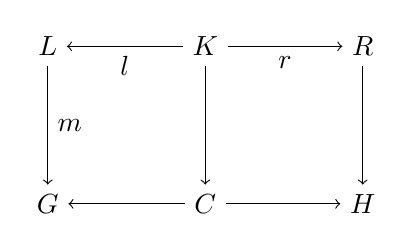
\begin{tikzpicture}
            \node (I) at (0,0) {$K$};
            \node (L)  at (-2,0) {$L$};
            \node (R)  at (2,0) {$R$};
            \node (G)  at (-2,-2) {$G$};
            \node (C)  at (0,-2) {$C$};
            \node (H)  at (2,-2) {$H$};
            \draw [->] (I) to  node [midway,below] {$l$} (L);
            \draw [->] (I) to  node [midway,below] {$r$} (R);
            \draw [->] (L) to node [midway,right] {$m$} (G);
            \draw [->] (I) to  node [midway,right] 
            % {$u$}
            {} (C); 
            \draw [->] (R) to  node [midway,right] 
            {}
            (H);
            \draw [->] (C) to node [midway,above] {} (G);
            \draw [->] (C) to node [midway,above] 
            {} 
            (H);
        \end{tikzpicture}
        }
    \end{center}
%         \caption{}
%         \label{fig:preliminaries:a_gadsfsddfsmework}
% \end{figure}

However, given a match $L \overset{m}{\rightarrow} G$, the left pushout square cannot always be constructed. For example, consider the same rewriting rule 
\begin{center}
      \resizebox{\textwidth}{!}{
      \begin{tikzpicture}
          \graphbox{$L$}{0mm}{0mm}{34mm}{15mm}{2mm}{-5mm}{
              \coordinate (o) at (0mm,-3mm); 
              \node[draw,circle] (l1) at ($(o)+(-10mm,0mm)$) {1};
              \node[draw,circle] (l2) at ($(l1)+(2,0)$) {2};
              \node[draw,circle] (l3) at ($(l1)+(1,0)$) {3};
              \draw[->] (l1) -- (l3) node[midway,above] {$a$};
              \draw[->] (l3) -- (l2) node[midway,above] {$a$};
          }     
          \graphbox{$K$}{40mm}{0mm}{24mm}{15mm}{2mm}{-5mm}{
              \coordinate (o) at (5mm,-3mm); 
              \node[draw,circle] (l1) at ($(o)+(-10mm,0mm)$) {1};
              \node[draw,circle] (l2) at ($(l1)+(1,0)$) {2};
              % \node[draw,circle] (l3) at ($(l1)+(1,0)$) {$\ $};
              % \draw[->] (l1) -- (l3) node[midway,above] {$a$};
              % \draw[->] (l3) -- (l2) node[midway,above] {$a$};
          }    
          \graphbox{$R$}{70mm}{0mm}{45mm}{15mm}{2mm}{-5mm}{
              \coordinate (o) at (-5mm,-3mm); 
              \node[draw,circle] (l1) at ($(o)+(-10mm,0mm)$) {1};
              \node[draw,circle] (l2) at ($(l1)+(3,0)$) {2};
              \node[draw,circle] (l3) at ($(l1)+(1,0)$) {4};
              \node[draw,circle] (l4) at ($(l1)+(2,0)$) {5};
              \draw[->] (l1) -- (l3) node[midway,above] {$a$};
              \draw[->] (l3) -- (l4) node[midway,above] {$b$};
              \draw[->] (l4) -- (l2) node[midway,above] {$a$};
          }    
          \node () at (37mm,-8mm) {$\overset{l}{\leftarrowtail}$};
          \node () at (67mm,-8mm) {$\overset{r}{\rightarrowtail}$};
          % \draw[>->] (51mm,2mm) -- (52mm,3mm);
      \end{tikzpicture}
      }
\end{center} 
%       \caption{}
%       \label{fig:preliminaries:a_rewrdfagiting_rule_sfdsgdfa}
%   \end{figure}
and the graph $G$ shown below:
\begin{center}
    \resizebox{0.4\textwidth}{!}{
\begin{tikzpicture}
        \graphbox{\( \mathcal{G} \)}{0mm}{-22mm}{34mm}{22mm}{2mm}{-3mm}{
                    \coordinate (o) at (0mm,-3mm); 
                    \node[draw,circle] (l1) at ($(o)+(-10mm,0mm)$) {$1$};
                    \node[draw,circle] (l2) at ($(l1)+(2,0)$) {$2$};
                    \node[draw,circle] (l3) at ($(l1)+(1,0)$) {$3$};
                    \node[draw,circle] (l4) at ($(l2)+(0,-1)$) {$6$};
                    \draw[red] (l3) -- (l4) node[midway,above] {$b$};
                    \draw (l1) -- (l3) node[midway,above] {$a$};
                    \draw (l3) -- (l2) node[midway,above] {$a$};
                    \draw (l2) -- (l4) node[midway,right] {$b$};
                    \node[draw,circle] (l6) at ($(l1)+(0,-1)$) {$7$};
                    \draw (l1) -- (l6) node[midway,left] {$b$};
                    % \draw[->] (l2) edge[out=-135,in=-45]node[midway,below] {$a$} (l1) ;
                }   
    \end{tikzpicture}
    }
\end{center}
The left pushout square cannot be constructed as visualized by the following figure, where the numbers inside nodes and the subgraphs in different colors illustrate how the morphisms map nodes and edges; the dashed circle in the box $C$ indicates that the node 3 is missing.

        \begin{center}
        \resizebox{\textwidth}{!}{
            \begin{tikzpicture}
                \graphbox{\( L \)}{0mm}{-3mm}{34mm}{12mm}{2mm}{2mm}{
                    \coordinate (o) at (0mm,-8mm); 
                    \node[draw,circle] (l1) at ($(o)+(-10mm,0mm)$) {1};
                    \node[draw,circle] (l2) at ($(l1)+(2,0)$) {2};
                    \node[orange,draw,circle] (l3) at ($(l1)+(1,0)$) {3};
                    \draw[orange,->] (l1) -- (l3) node[midway,above] {$a$};
                    \draw[orange,->] (l3) -- (l2) node[midway,above] {$a$};
                } 
        
                \graphbox{\( K \)}{40mm}{-3mm}{34mm}{12mm}{2mm}{2mm}{
                    \coordinate (o) at (0mm,-8mm); 
                    \node[draw,circle] (l1) at ($(o)+(-10mm,0mm)$) {1};
                    \node[draw,circle] (l2) at ($(l1)+(2,0)$) {2};
                }  
        
                \graphbox{\( R \)}{80mm}{-3mm}{45mm}{12mm}{2mm}{2mm}{
                    \coordinate (o) at (-5mm,-8mm); 
                    \node[draw,circle] (l1) at ($(o)+(-10mm,0mm)$) {1};
                    \node[draw,circle] (l2) at ($(l1)+(3,0)$) {2};
                    \node[draw,circle] (l3) at ($(l1)+(1,0)$) {4};
                    \node[draw,circle] (l4) at ($(l1)+(2,0)$) {5};
                    \draw[->] (l1) -- (l3) node[midway,above] {$a$};
                    \draw[->] (l3) -- (l4) node[midway,above] {$b$};
                    \draw[->] (l4) -- (l2) node[midway,above] {$a$};
                }    
        
                \graphbox{\( G \)}{0mm}{-22mm}{34mm}{22mm}{2mm}{-3mm}{
                    \coordinate (o) at (0mm,-3mm); 
                    \node[draw,circle] (l1) at ($(o)+(-10mm,0mm)$) {1};
                    \node[draw,circle] (l2) at ($(l1)+(2,0)$) {2};
                    \node[draw,circle,orange] (l3) at ($(l1)+(1,0)$) {3};
                    \node[blue, draw,circle] (l4) at ($(l2)+(0,-1)$) {6};
                    \draw[orange,->] (l1) -- (l3) node[midway,above] {$a$};
                    \draw[orange,->] (l3) -- (l2) node[midway,above] {$a$};
                    \draw[blue,->] (l2) -- (l4) node[midway,right] {$a$};
                    \node[blue,draw,circle] (l6) at ($(l1)+(0,-1)$) {7};
                    \draw[blue,<-] (l1) -- (l6) node[midway,left] {$a$};
                    \draw[->,red] (l3) -- (l4) node[midway,above] {$a$};
                }    
        
                \graphbox{\( C \)}{40mm}{-22mm}{34mm}{22mm}{2mm}{-3mm}{
                    \coordinate (o) at (0mm,-3mm); 
                    \node[draw,circle] (l1) at ($(o)+(-10mm,0mm)$) {1};
                    \node[draw,circle] (l2) at ($(l1)+(2,0)$) {2};
                    \node[blue,draw,circle] (l4) at ($(l2)+(0,-1)$) {6};
                    \draw[blue,->] (l2) -- (l4) node[midway,right] {$a$};
                    \node[blue,draw,circle] (l6) at ($(l1)+(0,-1)$) {7};
                    \draw[blue,<-] (l1) -- (l6) node[midway,left] {$a$};
                    \node[draw,circle,dashed,orange] (l3) at ($(l1)+(1,0)$) {3};
                    \draw[->,red] (l3) -- (l4) node[midway,above] {$a$};
                }    
                \node () at (37mm,-8mm) {\( \overset{l}{\leftarrowtail} \)}; % K -> L
                \node () at (77mm,-8mm) {\( \overset{r}{\rightarrowtail} \)}; % K -> R
                \node () at (15mm,-18mm) {\(m\ \downarrowtail \)};
                % \node () at (37mm,-33mm) {\( \leftarrowtail \)};
            %   \node () at (52mm,-18mm) {\( \downarrowtail \)};
            \end{tikzpicture}
        }       
        \end{center}
\noindent Specifically, the graph $G$ has the occurrence \raisebox{2pt}{
            \scalebox{0.7}{\tikz[baseline=-0.5ex]{
            \node [draw,circle] (z) at (-1,0) {$1$};
            \node [draw,circle] (x) at (0,0) {$3$};
            \node[draw,circle] (y) at (1,0) {$2$};
            \draw[->] (z)--(x) node[midway, above] {$a$};
            \draw[->] (x)--(y) node[midway, above] {$a$};
        }}} of $L$. Nevertheless, since node $3$ does not exist in $C$, the edge from node $3$ to node $6$ becomes dangling, making the construction of $C$ impossible and preventing the rule application on that occurrence of $L$. Concretely, nodes in \(m(L)\mathop{\setminus} (l\star m)(K)\) are removed when the rule is applied, while edges in \(G\mathop{\setminus} m(L)\) remain, which can produce dangling edges.
        Therefore, no node of $G$ outside the image of \(m\) should be incident to a node of \(m(L)\) outside the image of \(l\star m\). This requirement is precisely the dangling-edge condition in the following Proposition~\ref{prop:existence_of_pushout_complement}.

There is another requirement for the existence of a pushout complement. To give an intuition, consider the rewriting rule in \(\mathbf{Graph}\), shown below. 
    \begin{center}
        \resizebox{\textwidth}{!}{
            \begin{tikzpicture}
                \graphbox{\( L \)}{0mm}{-3mm}{34mm}{12mm}{2mm}{2mm}{
                    \coordinate (o) at (0mm,-8mm); 
                    \node[draw,circle] (l1) at ($(o)+(-10mm,0mm)$) {1};
                    \node[draw,circle] (l2) at ($(l1)+(2,0)$) {2};
                    \node[draw,circle] (l3) at ($(l1)+(1,0)$) {3};
                } 
        
                \graphbox{\( K \)}{40mm}{-3mm}{34mm}{12mm}{2mm}{2mm}{
                    \coordinate (o) at (0mm,-8mm); 
                    \node[draw,circle] (l1) at ($(o)+(-10mm,0mm)$) {1};
                    \node[draw,circle] (l2) at ($(l1)+(2,0)$) {2};
                }  
        
                \graphbox{\( R \)}{80mm}{-3mm}{45mm}{12mm}{2mm}{2mm}{
                    \coordinate (o) at (-5mm,-8mm); 
                    \node[draw,circle] (l1) at ($(o)+(-10mm,0mm)$) {$1$};
                    \node[draw,circle] (l2) at ($(l1)+(3,0)$) {$2$};
                }  
        
                \node () at (37mm,-8mm) {\( \overset{l}{\leftarrowtail} \)}; % K -> L
                \node () at (77mm,-8mm) {\( \overset{r}{\rightarrowtail} \)}; % K -> R
            \end{tikzpicture}
        } 
        \end{center} 
This rule deletes a node of the graph, and the match identifies the three nodes of \(L\) with a single node of \(G\). 
Consider the match \(L \overset{m}{\rightarrow} G\) shown in the following diagram:    
    \begin{center}
        \resizebox{\textwidth}{!}{
            \begin{tikzpicture}
                \graphbox{\( L \)}{0mm}{-3mm}{34mm}{12mm}{2mm}{2mm}{
                    \coordinate (o) at (0mm,-8mm); 
                    \node[draw,circle] (l1) at ($(o)+(-10mm,0mm)$) {1};
                    \node[draw,circle] (l2) at ($(l1)+(2,0)$) {2};
                    \node[draw,circle] (l3) at ($(l1)+(1,0)$) {3};
                } 
        
                \graphbox{\( K \)}{40mm}{-3mm}{34mm}{12mm}{2mm}{2mm}{
                    \coordinate (o) at (0mm,-8mm); 
                    \node[draw,circle] (l1) at ($(o)+(-10mm,0mm)$) {1};
                    \node[draw,circle] (l2) at ($(l1)+(2,0)$) {2};
                }  
        
                \graphbox{\( R \)}{80mm}{-3mm}{45mm}{12mm}{2mm}{2mm}{
                    \coordinate (o) at (-5mm,-8mm); 
                    \node[draw,circle] (l1) at ($(o)+(-10mm,0mm)$) {$1$};
                    \node[draw,circle] (l2) at ($(l1)+(3,0)$) {$2$};
                }  
        
                \graphbox{\( G \)}{0mm}{-22mm}{34mm}{22mm}{2mm}{-3mm}{
                    \coordinate (o) at (0mm,-3mm); 
                    \node[draw,circle] (l1) at ($(o)+(0mm,-5mm)$) {$1\ 2\ 3$};
                }    
                \node () at (37mm,-8mm) {\( \overset{l}{\leftarrowtail} \)}; % K -> L
                \node () at (77mm,-8mm) {\( \overset{r}{\rightarrowtail} \)}; % K -> R
                \node () at (15mm,-18mm) {\(m\ \downarrow \)};
            \end{tikzpicture}
        } 
        \end{center}     
Since there are no edges, we may view these graphs as sets of nodes and compute the left pushout square explicitly, as in Example~\ref{ex:cat:posfjsdlkgja}. Suppose that the left pushout square exists—i.e., there is a graph \(C\) and morphisms \(u: K \mathop{\to} C\) and \(l': C \mathop{\to} G\) such that the following diagram is a pushout square:
\begin{center}
      \resizebox{0.3\textwidth}{!}{
      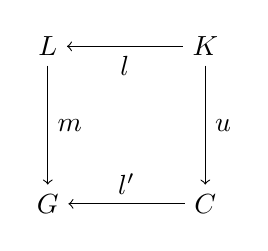
\begin{tikzpicture}
            \node (I) at (0,0) {$K$};
            \node (L)  at (-2,0) {$L$};
            \node (G)  at (-2,-2) {$G$};
            \node (C)  at (0,-2) {$C$};
            \draw [->] (I) to  node [midway,below] {$l$} (L);
            \draw [->] (L) to node [midway,right] {$m$} (G);
            \draw [->] (I) to  node [midway,right] {$u$} (C); 
            \draw [->] (C) to node [midway,above] {$l'$} (G);
        \end{tikzpicture}
        }
    \end{center}
Then the set of nodes of \(G\) is isomorphic to the quotient \(D/\!\sim\), where $D$ is the disjoint union of the set $V(L)$ of nodes of $L$ and the set $V(C)$ of nodes in $C$ and \(\sim\) is the equivalence relation generated by \(\set{(l(v),u(v))\mid v \mathop{\in} V(K)}\).
  
  In this example, there are two cases, depending on how the nodes of \(K\) map into \(C\). Throughout this paragraph, a node \(v\) of a graph \(X\) is denoted by \(v_X\) to avoid ambiguity. 
If nodes in $K$ are mapped to different nodes $1_C$ and $2_C$ in $C$, then
        $\sim$ is the smallest equivalence relation generated by $\set{(1_L,1_C),(2_L,2_C)}$ and $D \mathop{=} \set{1_L,2_L,3_L,1_C,2_C,\cdots}$.
If nodes in $K$ are mapped to the same node $1_C$ in $C$, 
then the equivalence relation $\sim$ is the smallest equivalence relation including $\set{(1_L,1_C),(2_L,1_C)}$ and $D \mathop{=} \set{1_L,2_L,3_L,1_C,\cdots}$.
In both cases \(3_L\notin[1_L]_\sim\), and \(G\) cannot be isomorphic to the quotient set \(D/\!\sim\), which contains at least two distinct elements. The condition that prevents this situation is the identification condition in Proposition~\ref{prop:existence_of_pushout_complement}.

This leads to the following proposition summarizing the conditions under which pushout complements exist.
\begin{proposition}[\cite{corradini1997algebraic}] 
    \label{prop:existence_of_pushout_complement}
    Let $K \overset{l}{\rightarrow} L$ and $L \overset{m}{\rightarrow} G$ be two morphisms in the category \textbf{Graph}. There are two morphisms $K \overset{u}{\rightarrow} C \overset{l'}{\rightarrow} G$ such that $K \overset{l}{\rightarrow} L \overset{m}{\rightarrow} G$ and $K \overset{u}{\rightarrow} L \overset{l'}{\rightarrow} G$ form a pushout square, as shown 
    below, 
    % in Figure~\ref{fig:preliminaries:a_pushout_square_complement} 
    if and only if the following conditions are satisfied:
    \begin{itemize} 
        \item{Dangling edge condition:} 
        No edge in \(G\mathop{\setminus} m(L)\) is incident to any node in \(m(L) \mathop{\setminus} (l \mathop{\star} m)(K)\);
        \item{Identification condition: } There is no $x,y \mathop{\in} L_V \mathop{\cup} L_E$ such that $x \mathop{\neq} y$, $m(x) \mathop{=} m(y)$ and $y \notin l(K_V \mathop{\cup} K_E)$.
    \end{itemize} 
    % \begin{figure}[H]
    %     \centering
    \begin{center}
        \resizebox{0.3\textwidth}{!}{
            \begin{tikzpicture}
                \node (I) at (0,0) {$K$};
                \node (L) at (-2,0) {$L$};
                \node (G) at (-2,-2) {$G$};
                \node (C) at (0,-2) {$C$};
                \draw [->] (I) to  node [midway,below] {$l$} (L);
                \draw [->] (L) to node [midway,right] {$m$} (G);
                \draw [->] (I) to node [midway,right] {$u$} (C);
                \draw [->] (C) to node [midway,above] {$l'$} (G);
                \node [at=($(I)!.5!(G)$)] {\normalfont PO};
            \end{tikzpicture}
        } 
        \end{center}
    %     \caption{}
    %     \label{fig:preliminaries:a_pushout_square_complement}
    % \end{figure}
\end{proposition}
 
%  In this example, edge $3 \overset{a}{\rightarrow} 6$ is in $G_E \mathop{\setminus} m(L_E)$, and it is incident to the node $3$ which is in $m(L_V \mathop{\setminus} l(K_V))$. When node $3$ is removed, the edge from node $3$ to node $6$ will be dangling. Intuitively, edges in $G_E \mathop{\setminus} m(L_E)$.

%     To give an intuition on the second condition, suppose that there is a graph C and morphisms $\beta$ and $\alpha'$ such that the diagram in Figure~\ref{fig:preliminaries:a_pushout_square_diagram_1} is a pushout square.
%    We have the commutative diagram in Figure~\ref{fig:preliminaries:a_pushout_square_diagram} where the morphism $\gamma$ maps all nodes in $C$ to the node 1 in $E$.

% \begin{figure}[H]
%     \centering
%         \resizebox{0.7\textwidth}{!}{
%         \begin{tikzpicture} 
%             \graphbox{\( L \)}{40mm}{20mm}{34mm}{20mm}{2mm}{2mm}{
%                 \coordinate (o) at (0mm,-8mm); 
%                 \node[draw,circle] (l1) at ($(o)+(-10mm,0mm)$) {1};
%                 \node[draw,circle] (l2) at ($(l1)+(2,0)$) {2};
%                 % \draw[->,red] (l2) edge[out=-135,in=-45]node[midway,below] {$a$} (l1) ;
%                 % \node[draw,circle,red] (l3) at ($(l1)+(1,0)$) {3};
%                 % \draw[->,red] (l1) -- (l3) node[midway,above] {$a$};
%                 % \draw[->,red] (l3) -- (l2) node[midway,above] {$a$};
%             } 
    
%             \graphbox{\( K \)}{0mm}{0mm}{34mm}{12mm}{2mm}{2mm}{
%                 \coordinate (o) at (0mm,-8mm); 
%                 \node[draw,circle] (l1) at ($(o)+(-10mm,0mm)$) {1};
%                 % \node[draw,circle] (l2) at ($(l1)+(2,0)$) {2};
%             }  
%             \graphbox{\(G  \)}{110mm}{5mm}{34mm}{40mm}{2mm}{-3mm}{
%                 \coordinate (o) at (0mm,-20mm); 
%                  \node[draw,circle] (l1) at ($(o)+(0,0)$) {1\ 2};
%                 % \node[draw,circle] (l1) at ($(o)+(-10mm,0mm)$) {1};
%                 % \node[draw,circle] (l2) at ($(l1)+(2,0)$) {2};
%                 % \draw[->,red] (l1) edge[loop below] node[midway, below] {$a$} (l1) ;
%                 % \node[draw,circle,red] (l3) at ($(l1)+(0,1.4)$) {3};
%                 % \node[draw,circle,blue] (l4) at ($(l1)+(1,-1)$) {6};
%                 % \draw[->,red] (l1) edge[bend left] node[midway,left] {$a$} (l3);
%                 % \draw[->,red] (l3) edge[bend left] node[midway,right] {$a$} (l1);
%                 % \draw[->,blue] (l1) edge  node[midway,right] {$a$} (l4);
%                 % \node[draw,circle,blue] (l6) at ($(l1)+(-1,-1)$) {7};
%                 % \draw[<-,blue] (l1) edge node[midway,left] {$a$} (l6) ;
%                 % \draw[->,blue] (l1) edge[out=-135,in=-45]node[midway,below] {$a$} (l1) ;
%             }   
%             \node () at (50mm,-28mm) {\( C \)};
%             % K to L  
%             \draw[->] (17mm,5mm) -- node[above] {$\alpha$} (37mm,15mm);
%             % C to G
%             \draw[->] (76mm,-28mm)-- node[below] {$\alpha'$} (104mm,-24mm) ;
%             % K to C
%             \draw[->] (17mm,-17mm) -- node[below] {$\beta$} (37mm,-28mm);
%             % L to G
%             \draw[->] (76mm,16mm) -- node[above] {$\beta'$} (104mm,7mm);
%             % \node () at (57mm,-6mm) {$PO$};
%         \end{tikzpicture}
%         }
%         \caption{}
%         \label{fig:preliminaries:a_pushout_square_diagram_1}
%     \end{figure} 
%    \begin{figure}[H]
%     \centering
%         \resizebox{0.7\textwidth}{!}{
%         \begin{tikzpicture} 
%             \graphbox{\( L \)}{40mm}{20mm}{34mm}{20mm}{2mm}{2mm}{
%                 \coordinate (o) at (0mm,-8mm); 
%                 \node[draw,circle] (l1) at ($(o)+(-10mm,0mm)$) {1};
%                 \node[draw,circle] (l2) at ($(l1)+(2,0)$) {2};
%                 % \draw[->,red] (l2) edge[out=-135,in=-45]node[midway,below] {$a$} (l1) ;
%                 % \node[draw,circle,red] (l3) at ($(l1)+(1,0)$) {3};
%                 % \draw[->,red] (l1) -- (l3) node[midway,above] {$a$};
%                 % \draw[->,red] (l3) -- (l2) node[midway,above] {$a$};
%             } 
    
%             \graphbox{\( K \)}{0mm}{0mm}{34mm}{12mm}{2mm}{2mm}{
%                 \coordinate (o) at (0mm,-8mm); 
%                 \node[draw,circle] (l1) at ($(o)+(-10mm,0mm)$) {1};
%                 \node[draw,circle] (l2) at ($(l1)+(2,0)$) {2};
%             }  
%             \graphbox{\(E \)}{110mm}{5mm}{45mm}{40mm}{2mm}{-3mm}{
%                 \coordinate (o) at (-10mm,-20mm); 
%                  \node[draw,circle] (l1) at ($(o)+(0,0)$) {1};
%                 % \node[draw,circle] (l1) at ($(o)+(-10mm,0mm)$) {1};
%                 \node[draw,circle] (l2) at ($(l1)+(2,0)$) {2};
%                 % \draw[->,red] (l1) edge[loop below] node[midway, below] {$a$} (l1) ;
%                 % \node[draw,circle,red] (l3) at ($(l1)+(0,1.4)$) {3};
%                 % \node[draw,circle,blue] (l4) at ($(l1)+(1,-1)$) {6};
%                 % \draw[->,red] (l1) edge[bend left] node[midway,left] {$a$} (l3);
%                 % \draw[->,red] (l3) edge[bend left] node[midway,right] {$a$} (l1);
%                 % \draw[->,blue] (l1) edge  node[midway,right] {$a$} (l4);
%                 % \node[draw,circle,blue] (l6) at ($(l1)+(-1,-1)$) {7};
%                 % \draw[<-,blue] (l1) edge node[midway,left] {$a$} (l6) ;
%                 % \draw[->,blue] (l1) edge[out=-135,in=-45]node[midway,below] {$a$} (l1) ;
%             }   
%             \node () at (50mm,-28mm) {\( C \)};
%             % K to L  
%             \draw[->] (17mm,5mm) -- node[above] {$\alpha$} (37mm,15mm);
%             % C to G
%             \draw[->] (76mm,-28mm)-- node[below] {$\gamma$} (104mm,-24mm) ;
%             % K to C
%             \draw[->] (17mm,-17mm) -- node[below] {$\beta$} (37mm,-28mm);
%             % L to G
%             \draw[->] (76mm,16mm) -- node[above] {$\gamma'$} (104mm,7mm);
%             % \node () at (57mm,-6mm) {$PO$};
%         \end{tikzpicture}
%         }
%         \caption{}
%         \label{fig:preliminaries:a_pushout_square_diagram}
%     \end{figure}
%     However, no morphism \(\delta : G \mathop{\to} E\) exists such that \( \gamma' \mathop{=} \beta' \mathop{\star} \delta \) and \( \gamma \mathop{=} \alpha' \mathop{\star} \delta \), which contradicts the universal property of the pushout. Therefore, there cannot be any graph \( C \) and morphisms \( \beta \) and \( \alpha' \) such that the diagram in the assumption is a pushout square.

There are several variants of DPO rewriting. Typically both the match $m$ and the morphism $l$ are required to be monomorphisms, and some variants impose additional constraints on the left pushout—for example, that the pushout complement be minimal or initial~\cite{braatz2011delete,behr2021concurrency,behr2023fundamentals}. Because these choices affect which rewriting steps are permitted and hence properties such as termination, following Endrullis and Overbeek~\cite{endrullis2024generalized_icgt}, we use the definition which is parametric in the variation of DPO under consideration.
\begin{definition}[\cite{endrullis2024generalized_icgt}]
  \label{def:rewriting_framework} 
    % A \textbf{DPO rewriting framework} $\mathfrak{F}$ is a funtion that to every rewriting rule \( \rho \mathop{=} (L \overset{l}{\leftarrow} K \overset{r}{\rightarrow} R) \) associates DPO diagrams as shown below
    A \textbf{DPO rewriting framework} $\mathfrak{F}$ is a mapping of DPO rewriting rules to classes of DPO diagrams. Specifically, for every rule \( \rho \mathop{=} (L \overset{l}{\leftarrow} K \overset{r}{\rightarrow} R) \), class $\mathfrak{F}(\rho)$ consists of DPO diagrams shown below, which are witnesses of rewriting steps using the rule \( \rho \).
%  \begin{figure}[H]
%       \centering
\begin{center}
      \resizebox{0.5\textwidth}{!}{
      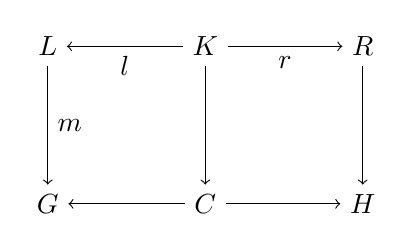
\begin{tikzpicture}
            \node (I) at (0,0) {$K$};
            \node (L)  at (-2,0) {$L$};
            \node (R)  at (2,0) {$R$};
            \node (G)  at (-2,-2) {$G$};
            \node (C)  at (0,-2) {$C$};
            \node (H)  at (2,-2) {$H$};
            \draw [->] (I) to  node [midway,below] {$l$} (L);
            \draw [->] (I) to  node [midway,below] {$r$} (R);
            \draw [->] (L) to node [midway,right] {$m$} (G);
            \draw [->] (I) to  node [midway,right] 
            % {$u$}
            {} (C); 
            \draw [->] (R) to  node [midway,right] 
            {}
            (H);
            \draw [->] (C) to node [midway,above] {} (G);
            \draw [->] (C) to node [midway,above] 
            {} 
            (H);
        \end{tikzpicture}
        }
    \end{center}
%         \caption{}
%         \label{fig:preliminaries:a_rewriting_framework}
% \end{figure}
    The \textbf{DPO rewriting relation $\mathop{\Rightarrow}_{\rho,\mathfrak{F}}$ induced by a DPO rewriting rule $\rho$ in $\mathfrak{F}$} is defined as follows:
     $$G \mathop{\Rightarrow}_{\rho,\mathfrak{F}} H\text{ if and only if }G \mathop{\Rightarrow}_\rho^\delta H$$
    for some $\delta \mathop{\in} \mathfrak{F}(\rho)$. 
     
    The \textbf{DPO rewriting relation $\mathop{\Rightarrow}_{\mathcal{R},\mathfrak{F}}$ induced by a set $\mathcal{R}$ of DPO rewriting rules in $\mathfrak{F}$} is given by: 
     $$G \mathop{\Rightarrow}_{\mathcal{R},\mathfrak{F}} H\text{ if and only if }G \mathop{\Rightarrow}_{\rho,\mathfrak{F}} H$$ for some $\rho \mathop{\in} \mathcal{R}$. 
     
     Whenever $\mathfrak{F}$ is clear from the context, we 
    omit $\mathfrak{F}$ and 
    write $\mathop{\Rightarrow}_{\rho}$ and $\mathop{\Rightarrow}_{\mathcal{R}}$.
  \end{definition}
% Let \(\mathfrak{F}\) denote the DPO rewriting framework that associates each rule \( \rho \mathop{=} (L \overset{l}{\leftarrow} K \overset{r}{\rightarrow} R) \) with the collection of all DPO diagrams of the form shown in Figure~\ref{fig:preliminaries:a_rewriting_framework}.
Hereafter, \(\mathfrak{M}\) denotes the DPO rewriting framework that associates each rule with the class of all DPO diagrams of the form shown in Definition~\ref{def:rewriting_framework} with monic match $m$.
